\chapter{Basics}\label{ch:basics}
The goal of this chapter is to introduce the reader to the mathematical fundamentals underlying the system developed. Obviously, it will be a brief overview, therefore, references to literature are provided if the reader would like to go more in detail with the proposed concepts.

\section{Least Square SLAM}\label{sec:ls_formulation}
In this section it proposed an insight of least-squares state estimation of non-linear stationary systems \cite{charnes1976least-squares}.

Suppose to have a stationary system $\mathcal{W}$ whose state is parametrized by a set of $N$ non-observable \textbf{state} variables $\mathbf{x} = \{\mathbf{x}_1, ..., \mathbf{x}_N\}$. Suppose that it is possible to indirectly observe the system state with different generic sensors, those will generate a set of $K$ \textbf{measurements} represented by $\mathbf{z} = \{\mathbf{z}_1, ..., \mathbf{z}_K\}$, where $\mathbf{z}_k$ is intended to be the $k^{th}$ measurement. Since the measurements are affected by noise, those are assumed to be \textbf{random variables}. Moreover, the state embeds all the knowledge needed to predict the measurements' distribution.

Since measurements are affected by noise, it is impossible to compute the state given the measurements. What is possible to evaluate, instead, is the states' distribution known the measurements, which can be formalized as following \textit{conditional probability}:

\begin{align} 
    p\left(\state | \meas\right) &= p\left(\state_1, ..., \state_N | \meas_1, ..., \meas_K\right) = \nonumber \\
    &= p\left(\state_{1:N} | \meas_{1:K}\right)
    \label{eq:cond_state_p}
\end{align}

The probability distribution \ref{eq:cond_state_p} is complex to retrieve in close form, for several reasons: 
\begin{itemize}
    \item The mapping between measurements and states can be highly non-linear, producing a multi-modal probability distribution with a complex shape.
    \item Each measurement $\meas_k$ in general observes only a subset of the state parameters. Moreover, the number of measurements may not be sufficient to fully characterize the state distribution.
    \item Measurements can be wrong - generating outliers - or it is impossible to map any of the state variable to a specified measurement.
\end{itemize}

However, what is possible to compute more easily is an estimate of the probability \ref{eq:cond_state_p}. To do so, we analyze the conditional distribution $p\left(\meas_k | \state\right)$: this is a predictive distribution called \textit{sensor model} or \textit{observation model}, which formalizes the probability of having a certain measurement \textit{assuming to know system's state}. Extending this to all the measurements, you will get the following distribution:

\begin{equation}
    p\left(\mathbf{z} | \mathbf{x}\right) = p\left(\meas_{1:K} | \state_{1:N}\right)
    \label{eq:likelihood}
\end{equation}

As it has been stated before, the state fully describes the measurements, rendering the single distributions $p\left(\mathbf{z}_k | \mathbf{x}\right)$ independent from each other. Exploiting this feature, it is possible to rewrite the \ref{eq:likelihood} as follows:

\begin{equation}
    \label{eq:obs_model_product}
    p\left(\meas_{1:K} | \state_{1:N}\right) = 
        \prod_{k = 1}^{K} p\left(\meas_k | \state_{1:N}\right)
\end{equation}

The equation \ref{eq:obs_model_product} describes the measurements' \textit{likelihood} given the state. Recalling the Bayes rule \cite{bayes-theorem} and applying it to \ref{eq:cond_state_p} you will obtain the following relation:

\begin{align*}
    p\left(\state_{1:N} | \meas_{1:K}\right) &= \frac{\overbracket{p\left(\meas_{1:K} | \state_{1:N}\right)}^{likelihood} \overbracket{p\left(\state_{1:N}\right)}^{prior}}{\underbracket{p\left(\meas_{1:K}\right)}_{normalizer}} = \\
    &= \frac{\prod_{k = 1}^{K} p\left(\meas_k | \state_{1:N}\right) p_x}{p_z} = \\
    &= \eta_{z} p_x \prod_{k = 1}^{K} p\left(\meas_k | \state_{1:N}\right)
\end{align*}

\noindent In this relation, $p\left(\state_{1:N}\right)$ represents our prior knowledge about the state distribution and, thus, supposing to know nothing about it, it is represented by a uniform distribution whose value is a constant $p_x$. $p\left(\meas_{1:K}\right)$ instead is just a normalizer for the overall probability function and does not depend from the states, therefore it is assumed to be a constant $p_z$. This leads to the following relation:

\begin{empheq}[box={\mybluebox[0pt]}]{equation}
    p\left(\state_{1:N} | \meas_{1:K}\right) \propto \prod_{k = 1}^{K} p\left(\meas_k | \state_{1:N}\right) 
    \label{eq:probability_proportionality}
\end{empheq}

\noindent Equation \ref{eq:probability_proportionality} represents the core of the entire least-square formulation. This will be exploited in the next subsections to approximate the distribution of interest, minimizing a defined cost function.

\subsection{Direct Minimization}\label{sec:direct_minimization}
Starting from the relation \ref{eq:probability_proportionality} it is possible to initialize a minimization problem. Assuming that the measurement are affected by \textit{Additive White Gaussian Noise}, the observation model probability $p\left(\meas_k | \state_{1:N}\right)$ will be described by a Gaussian distribution $\mathcal{N}(\mu, \Omega^{-1})$, leading to the equation

\begin{equation}
    p\left(\meas_k | \state_{1:N}\right) \propto \exp\left(-(\pred_k - \meas_k) \Omega_k(\pred_k - \meas_k)\right)
    \label{eq:obs_model_probability}
\end{equation}

\noindent where $\pred_k$ is the \textbf{prediction} of the measurement given the state, while $\Omega_k = \Sigma_k^{-1}$ represents conditional measurement's information matrix. The predicted measurement $\pred_k$ is a function of the state; in particular it is obtained applying the \textbf{sensor model} $h_k(\cdot)$ to the state, in formul\ae:

\begin{equation}
    \pred_k = h_k(\state)
    \label{eq:prediction}
\end{equation}

\noindent In SLAM - and other similar problems like SfM - the sensor model is a highly non-linear function, making the problem more complex and heavy from a computational point of view. Nevertheless, generally the sensor model is smooth enough to be approximated with its \textit{first-order Taylor expansion} in the neighbor of a linearization point $\linstate$, leading to:

\begin{empheq}[box={\mybluebox[0pt]}]{equation}
    h_k(\linstate + \dx) \approx h_k(\linstate) + \frac{\partial h_k(\state)}{\partial \state} \bigg\rvert_{\state = \linstate} \dx = h_k(\linstate) + \jacob_k \dx
    \label{eq:linearization}
\end{empheq}

\noindent where $\jacob_k = \frac{\partial h_k(\state)}{\partial \state} \bigg\rvert_{\state = \linstate}$ is the \textit{Jacobian} evaluated in $\state = \linstate$.

The next step consists in finding a linearization point $\optstate$ that \textit{maximizes the observation model}, leading to the following relations:

\begin{align*}
    \optstate 	&= \argmax_\state p(\meas | \state) =\\
                &= \argmax_\state \prod_{k = 1}^{K}p(\meas_k | \state) =\\
                &= \argmax_\state \prod_{k = 1}^{K}\exp\left(-(h_k(\state) - \meas_k)^T\Omega_k(h_k(\state) - \meas_k)\right) =\\
                &= \argmin_\state \sum_{k = 1}^{K} \left((h_k(\state) - \meas_k)^T\Omega_k(h_k(\state) - \meas_k)\right)
\end{align*}

\noindent The relation $\error_k(\state) = h_k(\state) - \meas_k$ represents the \textit{error function}, and, thus, the optimal linearization point will be given by the minimization of the following \textit{cost function}:

\begin{equation}
    F(\state) = \sum_{k = 1}^ {K} \underbracket{\error_k^T(\state)\Omega_k\error_k(\state)}_{\error_k(\state)}
    \label{eq:cost_function}
\end{equation}

\noindent In order to find the optimum linearization point, the system must start from a reasonable initial guess $\linstate$ - to avoid local minima - and apply an increment $\dx$ directed toward $\optstate$. Applying the perturbation $\dx$ in the error function and approximating again through the first-order Taylor expansion we will obtain 

\begin{align}
    \error_k(\linstate + \dx) &= \left(h_k(\linstate + \dx) - \meas_k)^T \Omega_k (h_k(\linstate + \dx) - \meas_k)\right) =\nonumber\\
    &\approx (\jacob_k\dx + h_k(\linstate) - \meas_k)^T \Omega_k (\jacob_k\dx + h_k(\linstate) - \meas_k) =\nonumber\\
    &= (\jacob_k\dx + \error_k(\linstate))^T \Omega_k (\jacob_k\dx + \error_k(\linstate))
    \label{eq:error_perturbation}
\end{align}

\noindent Further expanding the quantities in the equation \ref{eq:error_perturbation}, it is possible to obtain the following relation:

\begin{align}
    \error_k(\linstate + \dx) &\approx \dx^T\overbracket{\jacob_k^T\Omega_k\jacob_k}^{H_k}\dx + 2\,\overbracket{\jacob_k^T\Omega_k\error_k(\linstate)}^{\mathbf{b}_k}\,\dx + \overbracket{\error_k^T(\linstate)\Omega_k\error_k(\linstate)}^{\mathbf{c}_k} =\nonumber\\
    &= \dx^TH_k\dx + 2\,\mathbf{b}_k\dx + \mathbf{c}_k
    \label{eq:quadratic_form_k}
\end{align}

Extending the perturbation to the total cost function expressed in equation \ref{eq:cost_function} and plugging what stated in \ref{eq:quadratic_form_k} we will obtain:

\begin{align}
    F(\linstate + \dx) &\approx \sum_{k = 1}^{K} \left[\dx^TH_k\dx + 2\,\mathbf{b}_k\dx + \mathbf{c}_k\right] =\nonumber\\
    &= \dx^T\,\underbracket{\left[\sum_{k = 1}^KH_k\right]}_{\hessian}\dx + 2\,\underbracket{\left[\sum_{k = 1}^K\mathbf{b}_k\right]}_{\mathbf{b}}\dx + \underbracket{\sum_{k = 1}^K\mathbf{c}_k}_{\mathbf{c}} \nonumber = \\
    &= \dx^T\hessian\dx + 2\,\mathbf{b}\dx + \mathbf{c}
    \label{eq:quadratic_form}
\end{align}

It is good to notice that equation \ref{eq:quadratic_form} represents a \textit{quadratic form} in $\dx$. Thus, finding the minimum of this formula will give us the optimal perturbation $\dx$ such that

\begin{equation*}
    \optstate = \linstate + \dx
\end{equation*}

\noindent In order to find the minimum of equation \ref{eq:quadratic_form} we derive it in $\dx$, we equal the derivative to zero and finally we solve the resulting equation for $\dx$; in formul\ae:

\begin{equation}
    \frac{\partial\left(\dx^T\hessian\dx + 2\,\mathbf{b}\dx + \mathbf{c}\right)}{\partial \dx} = 2\,\hessian\dx + 2\,\mathbf{b} = 0
    \label{eq:quatratic_form_derivative}
\end{equation}

\noindent Therefore, in order to find the solution of equation \ref{eq:quatratic_form_derivative} and finally get to the optimal perturbation, we must solve the following \textit{linear system}:

\begin{empheq}[box={\mybluebox[0pt]}]{equation}
\hessian\,\dx^\star = -\mathbf{b}
\label{eq:linear_system}
\end{empheq}


\begin{algorithm}
    \label{alg:gn_standard}
    \caption{Standard Gauss-Newton minimization algorithm}
    \begin{algorithmic}[1]
        \Require{Initial guess $\linstate$; a set of measurements $\mathcal{C} = \{\langle\meas_k, \Omega_k\rangle\}$}
        \Ensure{Optimal solution $\state^\star$}
        \vspace{10px}
        \State $F_{new} \leftarrow \breve{F}$ \Comment{compute the current error}
        \vspace{5px}
        \While{$\breve{F} - F_{new} > \epsilon$}
            \State $\breve{F} \leftarrow F_{new}$
            \State $\mathbf{b} \leftarrow 0$
            \State $\hessian \leftarrow 0$
            \vspace{5px}
            \ForAll{$k \in \{1, ..., K\}$}
                \State $\pred_k \leftarrow h_k(\linstate)$ \Comment{compute prediction}
                \State $\error_k \leftarrow \pred_k - \meas_k$ \Comment{compute error}
                \State $\jacob_k \leftarrow \frac{\partial h_k(\state)}{\partial \state} \bigg\rvert_{\state = \linstate}$ \Comment{compute Jacobian}
                
                \State $\hessian_k \leftarrow \jacob_k^T\Omega_k\jacob_k$ \Comment{contribution of $\meas_k$ in $\hessian$}
                \State $\mathbf{b}_k \leftarrow \jacob_k^T\Omega_k\error_k$ \Comment{contribution of $\meas_k$ in $\mathbf{b}$}
                
                \State $\hessian \pluseq \hessian_k$ \Comment{Accumulate contributions in $\hessian$}
                \State $\mathbf{b} \pluseq \mathbf{b}_k$ \Comment{Accumulate contributions in $\mathbf{b}$}
            \EndFor
            \vspace{5px}
            \State $\dx \leftarrow solve(\hessian\dx = -\mathbf{b})$ \Comment{Solve linear system}
            \State $\linstate \pluseq \dx $ \Comment{Apply increment}
            \State $F_{new} \leftarrow F(\linstate)$ \Comment{Update the error}
        \EndWhile
        \vspace{5px}
        \State \Return $\linstate$
    \end{algorithmic}
\end{algorithm}

It is good to notice that, if the \textit{sensor model} $h_k(\cdot)$ is a linear function of the state, it is possible to find the minimum in just one iteration. However, since it is almost never the case in our cases of study, a solution must be found iteratively, until convergence is reached. To do so, it is possible to use the \textbf{Gauss-Newton} algorithm - described in \hyperref[alg:gn_standard]{Algorithm 1}. However, \textit{Gauss-Newton} is not guaranteed to converge in general. The convergence is subject to several factors, like the smoothness of the error function used or the initial guess - i.e. if it is close to potential singularity or far from the optimal solution. \textit{Levenberg-Marquardt} iterative algorithm is variation of \textit{Gauss-Newton} that enforces the convergence - shown in detail in \hyperref[alg:lm_standard]{Algorithm 2}. It solves a \textit{damped} version of the linear system \ref{eq:linear_system}, described by the following formula:

\begin{equation}
    \left(\hessian + \lambda\mathbf{I}\right)\dx = -\mathbf{b}
    \label{eq:lm_algorithm}
\end{equation} 

\noindent where $\lambda$ is a scalar \textit{damping} factor. The algorithm does not diverge, but it may converge to a \textit{local minimum} and, thus, retrieving a sub-optimal solution. 


\begin{algorithm}[!h]
    \label{alg:lm_standard}
    \caption{Standard Levenberg-Marquardt minimization algorithm}
    \begin{algorithmic}[1]
        \Require{Initial guess $\linstate$; a set of measurements $\mathcal{C} = \{\langle\meas_k, \Omega_k\rangle\}$}
        \Ensure{Optimal solution $\state^\star$}
        \vspace{10px}
        \State $F_{new} \leftarrow \breve{F}$ \Comment{compute the current error}
        \State $\state_{backup} \leftarrow \linstate$ \Comment{backup the solution}
        \State $\lambda \leftarrow \text{computeInitialLambda}(\mathcal{C}, \linstate)$
        \vspace{5px}
        \While{$\breve{F} - F_{new} > \epsilon \wedge t < t_{max}$}
        \State $\breve{F} \leftarrow F_{new}$
        \State $\mathbf{b} \leftarrow 0$
        \State $\hessian \leftarrow 0$
        \vspace{5px}
        \ForAll{$k \in \{1, ..., K\}$}
        \State $\pred_k \leftarrow h_k(\linstate)$ \Comment{compute prediction}
        \State $\error_k \leftarrow \pred_k - \meas_k$ \Comment{compute error}
        \State $\jacob_k \leftarrow \frac{\partial h_k(\state)}{\partial \state} \bigg\rvert_{\state = \linstate}$ \Comment{compute Jacobian}
        
        \State $\hessian_k \leftarrow \jacob_k^T\Omega_k\jacob_k$ \Comment{contribution of $\meas_k$ in $\hessian$}
        \State $\mathbf{b}_k \leftarrow \jacob_k^T\Omega_k\error_k$ \Comment{contribution of $\meas_k$ in $\mathbf{b}$}
        
        \State $\hessian \pluseq \hessian_k$ \Comment{accumulate contributions in $\hessian$}
        \State $\mathbf{b} \pluseq \mathbf{b}_k$ \Comment{accumulate contributions in $\mathbf{b}$}
        \EndFor
        
        \State $t \leftarrow 0$ \Comment{n. of iterations $\lambda$ has been adjusted}
        
        \vspace{5px}
        \While{$t < t_{max} \wedge t > 0$}
        \State $\dx \leftarrow solve\left((\hessian + \lambda I)\dx = \bvec\right)$ \Comment{solve damped linear system}
        \State $\linstate \pluseq \dx$ \Comment{apply increment}
        \State $F_{new} \leftarrow F(\linstate)$ \Comment{update the error}
        \If{$F_{new} < \breve{F}$}
        \State $\lambda \leftarrow \nicefrac{\lambda}{2}$ \Comment{good step, accept the solution}
        \State $\state_{backup} \leftarrow \linstate$
        \State $t \leftarrow t - 1$
        \Else
        \State $\lambda \leftarrow \lambda * 4$ \Comment{bad step, revert the solution}
        \State $\linstate \leftarrow \state_{backup}$
        \State $t \leftarrow t + 1$
        \EndIf
        \EndWhile
        \vspace{5px}
        
        \EndWhile
        \vspace{5px}
        \State \Return $\linstate$
    \end{algorithmic}
\end{algorithm}

It is good to notice that the system developed in this work uses the \textit{Gauss-Newton} algorithm, since the error function has been properly manipulated to be more linear with respect to other approaches. Obviously, more details can be found in the next Chapters.

\section{Manifolds}
In the previous Section it has been shown how to compute the optimal solution to the problem through Least-Squares estimation. However, two strong assumptions have been made:

\begin{enumerate}
    \item The measurement function is smooth enough to be approximated by its \textit{first-order Taylor expansion} without loss of generality
    \item The state space spans over an \textit{Euclidean domain}, and, thus $\state \in \mathbb{R}^n$
\end{enumerate}


\noindent While the first hypothesis is true in general, the second one is almost never verified in SLAM problems. For example, if the state of the system is the robot 3D-pose, it involves to deal \textit{Euler angles} or rotations in general; therefore the state belongs to $SE(3)$ - namely the \textit{Special Euclidean group} of dimension 3. In this topological spaces, operations like \textit{sum} or the \textit{product} are not defined as in $\mathbb{R}^n$, thus they are illegal - i.e. summing 2 triads of Euler angles will lead to an inconsistent result or to singular configurations.

However, in SLAM - as in SfM or BA - the state generally belongs to \textit{topological spaces} that \textit{locally resemble} the Euclidean space, called \textbf{manifolds}. This means that each point of an $n-$dimensional manifold has a neighborhood that is homeomorphic to $\mathbb{R}^n$. Examples of manifolds are spheres or toruses, which are \textit{locally} flat - the reader can think to the Earth that, for its inhabitants, seems flat.

Stepping back to our problem, it is possible for us to use this property to perform Least-Square estimation also with state spaces that are manifold. Assuming that our state belongs to $SO(3)$ - 3D rotations - if we represent it through a rotation matrix $\rot(\phi, \theta, \psi)$ it is not possible to simply sum two quantities since it is not enforced the matrix's orthogonality. A minimal representation, instead, $\state = (\phi, \theta, \psi)$ will lead to singularities. However, if we are in a neighborhood of the origin, Euler angles are away from singularities. Thus we can define an operator \textit{box-plus} that locally sums two quantities, exploiting manifold's property. The same must be done for other mathematical operators. In the case of rotation, we can define the following operators:

\begin{align}
    \label{eq:bp_rotations}
    \rot &= \rot_0 \boxplus \mathbf{u} = toMatrix(\mathbf{u})\, \rot_0\\
    \mathbf{u} &= \rot \boxminus \rot_0 = toEuler(\rot_0^{T} \, \rot)
    \label{eq:bm_rotations}
\end{align}

\noindent The operators $\boxminus$ and $\boxplus$ convert a global difference in the manifold into a local perturbation and vice versa.

Now we have to feed this new formalizations into the previously seen Least-Squares algorithm. From now on, $\SState$ indicates the over-parametrized representation of the state, while $\state$ the minimal one - i.e. a vector. Recalling the equation \ref{eq:linearization}, to linearize the problem it is necessary to apply a perturbation $\dx$ to the current estimate of the state $\Linstate$. However, to do so, it must be employed the new operator \textit{sum}. Moreover, $\Linstate$ can be treated as a constant since is the current estimate of the system; still, it is possible to span the state space by varying $\Delta\state$ (minimal representation). Therefore, the first order Taylor expansion of $h_k(\Linstate \boxplus \dx)$ is computed with respect to $\dx$, in the linearization point $\dx = 0$. This leads to the following new formulation:

\begin{empheq}[box={\mybluebox[5pt]}]{equation}
    h_k(\Linstate \boxplus \dx) \approx h_k(\Linstate) + \underbracket{\frac{\partial h_k(\SState \boxplus \dx)}{\partial \dx} \bigg\rvert_{\dx = 0}}_{\tjacob_k} \dx = h_k(\Linstate) + \tjacob_k \dx
    \label{eq:linearization_manifold}
\end{empheq}

\noindent It is good to notice that the formulation \ref{eq:linearization_manifold} is topologically similar to the equation \ref{eq:linearization} with obvious differences due to the manifold state space. 

As a consequence of what we have seen so far, in order to compute the optimal $\Linstate$, the operator $\boxplus$ must be used to apply the optimal increment, leading to the following relation:

\begin{equation}
    \SState^\star = \Linstate \boxplus \dx^\star
\end{equation}

Until now, it has been assumed that the measurements lie on $\mathbb{R}^n$. However, in our case of study, those may lie on a manifold too. This means that we have to define some new mathematical operators and minimal/redundant representations also for the measurements, like it has been done for the states. In particular, we know that the generic error function is $\error_k(x) = h_k(\state) - \meas_k$; now it is necessary to introduce the new operator \textit{difference}, that leads to the following error formulation:

\begin{equation}
    \terror_k(\SState) = \terror_k(\pred_k, \meas_k) = h_k(\SState) \boxminus \meas_k
    \label{eq:error_manifold}
\end{equation}

\noindent Equation \ref{eq:error_manifold} computes the error between the predicted measurement and the actual one in the minimal space, centering the computation in $\meas_k$. In general the error function will be smooth and regular even using the operator $\boxplus$, since the displacement between $h_k(\SState)$ and $\meas_k$ is generally small.

Applying a small perturbation $\dx$ to the \textit{prediction}, it is possible to compute the first order Taylor expansion of the error, which gives the following result:

\begin{align}
    \terror_k(\pred_k + \dz_k, \meas_k) &= (\pred_k + \dz_k) \boxminus \meas_k \approx \nonumber \\
    &\approx \pred_k \boxminus \meas_k + \underbracket{\frac{\partial\left((\pred_k + \dz_k) \boxminus \meas_k\right)}{\partial\dz_k}  \bigg\rvert_{\dz_k = 0}}_{\jacob_{\meas_k}} \dz_k
    \label{eq:error_linearization}
\end{align}

\noindent It is good to notice that the approximation of the error conditional distribution is described by a Gaussian with mean $\pred_k \boxminus \meas_k$ and covariance $\Sigma_{\error_k|\state} = \jacob_{\meas_k}\Omega_k^{-1}\jacob_{\meas_k}^T$. The reader must notice that projecting the measurement onto a minimal space using the operator $\boxminus$ makes the covariance of the conditional error distribution a function of the state - since it depends by $\pred_k$. Therefore, $\Sigma_{\error_k|\state}$ must be computed at every iteration. However, in our work we manged to keep the error function Euclidean, avoiding the computation of $\Sigma_{\error_k|\state}$ even if the measurements lie on $SE(3)$ - e.g. in the case of pose measurements like the ones generated by the odometry. 

In order to simplify the computation $\tjacob_k$ it is possible to exploit the chain rule for partial derivatives, which leads to following relation

\begin{equation}
    \frac{\partial\, \error_k\left(\linstate \boxplus \dx\right)}{\partial \dx} = \underbracket{\frac{\partial \error_k(\state)}{\partial \state} \bigg\rvert_{\state = \linstate}}_{\jacob_k} + \underbracket{\frac{\partial (\linstate \boxplus \dx)}{\partial \dx} \bigg\rvert_{\dx = 0}}_{\mathbf{M}}
    \label{eq:jacobian_chain_rule}
\end{equation}

\noindent where $\jacob_k$ is the simple Jacobian computed in the Euclidean case, while $\mathbf{M}$ represents the derivate of $\boxplus$ operator evaluated in $\linstate$. Given this, the total Jacobian $\tjacob_k$ computed on a manifold is described by the relation

\begin{empheq}[box={\mybluebox[0pt]}]{equation}
    \tjacob_k = \jacob_k \mathbf{M}
    \label{eq:jacobian_manifold}
\end{empheq}

Finally, it is possible to plug all this new elements in the modified version of the \textit{Gauss-Newton} algorithm - or the \textit{Levenberg-Marquardt} one - to perform the optimization process properly with non-euclidean states and measurements, explained in detail in \hyperref[alg:gn_manifolds]{Algorithm 3}.

\begin{algorithm}[h]
    \label{alg:gn_manifolds}
    \caption{Gauss-Newton minimization algorithm for manifold measurements and state spaces}
    \begin{algorithmic}[1]
        \Require{Initial guess $\linstate$; a set of measurements $\mathcal{C} = \{\langle\meas_k, \Omega_k\rangle\}$}
        \Ensure{Optimal solution $\state^\star$}
        \vspace{10px}
        \State $F_{new} \leftarrow \breve{F}$ \Comment{compute the current error}
        \vspace{5px}
        \While{$\breve{F} - F_{new} > \epsilon$}
            \State $\breve{F} \leftarrow F_{new}$
            \State $\mathbf{b} \leftarrow 0$
            \State $\hessian \leftarrow 0$
            \vspace{5px}
            \ForAll{$k \in \{1, ..., K\}$}
                \State $\pred_k \leftarrow h_k(\linstate)$ \Comment{compute prediction}
                
                \State $\error_k \leftarrow \pred_k \boxminus \meas_k$ \Comment{compute error with over-parametrized $\meas_k$}
                
                \State $\tjacob_k \leftarrow \frac{\partial \terror_k(h_k(\SState \boxplus \dx), \meas_k)}{\partial \dx_k} \bigg\rvert_{\dx_k = 0}$ \Comment{compute Jacobian of the error function}
                
                \State $\jacob_{\meas_k} \leftarrow \frac{\partial \left((\pred_k + \dz_k) \boxminus \meas_k\right)}{\partial \dz_k} \bigg\rvert_{\dz_k = 0}$ \Comment{compute Jacobian of the $\boxminus$ w.r.t. $\dz_k$}
                
                \State $\tilde{\Omega}_k \leftarrow \left(\jacob_{\meas_k}\Omega_k\jacob_{\meas_k}^{T}\right)^{-1}$ \Comment{Remap the information matrix}
                
                \State $\hessian_k \leftarrow \jacob_k^T\tilde{\Omega}_k\jacob_k$ \Comment{contribution of $\meas_k$ in $\hessian$}
                
                \State $\mathbf{b}_k \leftarrow \jacob_k^T\tilde{\Omega}_k\error_k$ \Comment{contribution of $\meas_k$ in $\mathbf{b}$}
                
                \State $\hessian \pluseq \hessian_k$ \Comment{Accumulate contributions in $\hessian$}
                \State $\mathbf{b} \pluseq \mathbf{b}_k$ \Comment{Accumulate contributions in $\mathbf{b}$}
            \EndFor
            \vspace{5px}
            \State $\dx \leftarrow solve(\hessian\dx = -\mathbf{b})$ \Comment{Solve linear system}
            \State $\linstate \leftarrow \linstate \boxplus \dx $ \Comment{Apply increment}
            \State $F_{new} \leftarrow F(\linstate)$ \Comment{Update the error}
        \EndWhile
        \vspace{5px}
        \State \Return $\linstate$
    \end{algorithmic}
\end{algorithm}

\section{Sparse Least Squares}\label{sec:sparse_ls}
In the previous Sections it has been introduced several powerful tools to estimate a set of hidden variables given a set of measurements that are related to those variables. However, the state vector - especially in SLAM applications - may easily become big and, thus, it creates a big bottleneck that kills the performances. Still, it is possible to overcome this dimensional problem exploiting the nature of the measurements. In fact, a single measurement $\meas_k$ depends only by a \textit{subset} $\state_k = \state_{r:s} = \{\state_r, ..., \state_s\} \subseteq \state_{1:N} $ of the whole state vector and this will lead to special structure of the \textit{Hessian} matrix $\hessian$.

Going deeper in this analysis, it is good to notice that each measurement contributes to the \textit{Hessian} $\hessian$ and the \textit{right-hand-side vector} $\bvec$ with just one addend - namely $\hessian_k$ and $\bvec_k$. The structure of those quantities depends by the Jacobian of the error function and this last one depends only by the state variables involved by the measurement. 

Recalling equations \ref{eq:linearization} and \ref{eq:jacobian_manifold} and on the basis of what just stated, \textit{Jacobian}'s structure will be:

\begin{equation}
    \jacob_k = \underbracket{\left[\zero \cdots \zero \: \jacob_{k_1} \zero \cdots \zero \: \jacob_{k_h} \zero \cdots \zero \: \jacob_{k_q} \zero \cdots \zero\right]}_{N blocks}
    \label{eq:sparse_jacobian}
\end{equation}

\noindent where each non-zero component $\jacob_{k_h} = \frac{\partial \error_k(\state_k)}{\partial \state_{k_h}}$ represents the partial derivative of the error function deriving from $\meas_k$, computed with respect to the parameter block $\state_{k_h} \in \state_k$. According to equation \ref{eq:quadratic_form_k}, the contribution to $\hessian$ and $\bvec$ will have the following anatomy:

\begin{align}
    \label{eq:sparse_hessian_structure}
    \hessian_k &= 
        \begin{pmatrix}
            \ddots &  &  &  &  &  &\\
             & \jacob_{k_1}^T\Omega_k\jacob_{k_1} & \cdots & \jacob_{k_1}^T\Omega_k\jacob_{k_h} & \cdots & \jacob_{k_1}^T\Omega_k\jacob_{k_q} & \\
             & \vdots & & \vdots & & \vdots & \\
             & \jacob_{k_h}^T\Omega_k\jacob_{k_1} & \cdots & \jacob_{k_h}^T\Omega_k\jacob_{k_h} & \cdots & \jacob_{k_h}^T\Omega_k\jacob_{k_q} & \\
             & \vdots & & \vdots & & \vdots & \\
             & \jacob_{k_q}^T\Omega_k\jacob_{k_1} & \cdots & \jacob_{k_q}^T\Omega_k\jacob_{k_h} & \cdots & \jacob_{k_q}^T\Omega_k\jacob_{k_q} & \\
             &  &  &  &  &  & \ddots \\
        \end{pmatrix} \\
    \bvec_k &= 
        \begin{bmatrix}
            \vdots \\
            \jacob_{k_1}\Omega_k\error_k \\
            \vdots \\
            \jacob_{k_h}\Omega_k\error_k \\
            \vdots \\
            \jacob_{k_q}\Omega_k\error_k \\
            \vdots
        \end{bmatrix}
    \label{eq:rhs_structure}
\end{align}

The internal structure of $\hessian$ and $\bvec$ just shown, reveals some important properties of those objects:

\begin{itemize}
    \item $\bvec$ is a \textbf{dense vector} composed by $N$ non-zero blocks. 
    \item The Hessian $\hessian$ is a \textbf{sparse symmetric matrix}.
    \item Every new measurement $q$ introduces $q^2$ non-zero blocks in the Hessian.
\end{itemize}

Hessian's sparsity is fundamental to perform efficient and fast optimization, especially to solve the linear system \ref{eq:linear_system}. The literature proposes many approaches to efficiently solve sparse linear systems, either with \textit{direct} \cite{davis2006directSPsolvers} or \textit{iterative} \cite{saad2003iterativeSPsolvers} methods. One of the most employed direct method uses the \textit{Cholesky} factorization of the matrix - namely the $LU$ decomposition. In this case, the Hessian is decomposed into two triangular matrices $\hessian = \mathbf{L}\mathbf{U}$, where $\mathbf{U} = \mathbf{L}^T$ and $\mathbf{L}$ is a \textit{lower-triangular matrix}. The solution to the original system is found solving consecutively the following derived systems:

\begin{equation}
    \label{eq:fwd_bwd_sub}
    \begin{cases}
        \mathbf{L}\,\mathbf{y} &= \bvec \\
        \mathbf{U}\,\dx &= \mathbf{y}
    \end{cases}
\end{equation}

\noindent Since $L$ and $U$ are triangular matrices, the solutions of equations \ref{eq:fwd_bwd_sub} can be easily computed through \textit{Forward} and \textit{Backward Substitution} respectively. It is good to notice that the \textit{Cholesky} decomposition of a sparse matrix will have a greater number of non-zero entries than the source, due to the \textit{fill-in} deriving from the decomposition itself. However, it is possible to reduce the \textit{fill-in} with several techniques, like \textit{variable reordering}. This is achieved pre and post-multiplying the source matrix - $\hessian$ - for a suitable \textit{permutation matrix} $\mathbf{P}$. The \textit{Cholesky} factorization will be applied to the permuted matrix $\mathbf{P}\hessian \mathbf{P}^T = \hat{\mathbf{L}}\hat{\mathbf{U}}$, preserving the sparsity and, thus, leading to faster solution of the linear system. 

The literature proposes a lot of theory on how to retrieve the good ordering to reduce the fill-in, minimize the \textit{FLOPs} or to exploit parallel computation. Some of the most effective orderings to reduce the fill-in are computed by \textit{Minimum Degree} \cite{amestoy1996amd, davis2004colamd}, \textit{super-nodal} \cite{cleveland1987supernodal} and \textit{nested dissection based} algorithms \cite{karypis1998metis}. It is good to notice that this is an \textit{NP-hard} problem and several libraries have been developed to compute orderings in a fast and efficient way \cite{agarwal2012variable}.

\begin{figure}[!hbt]
    \centering
    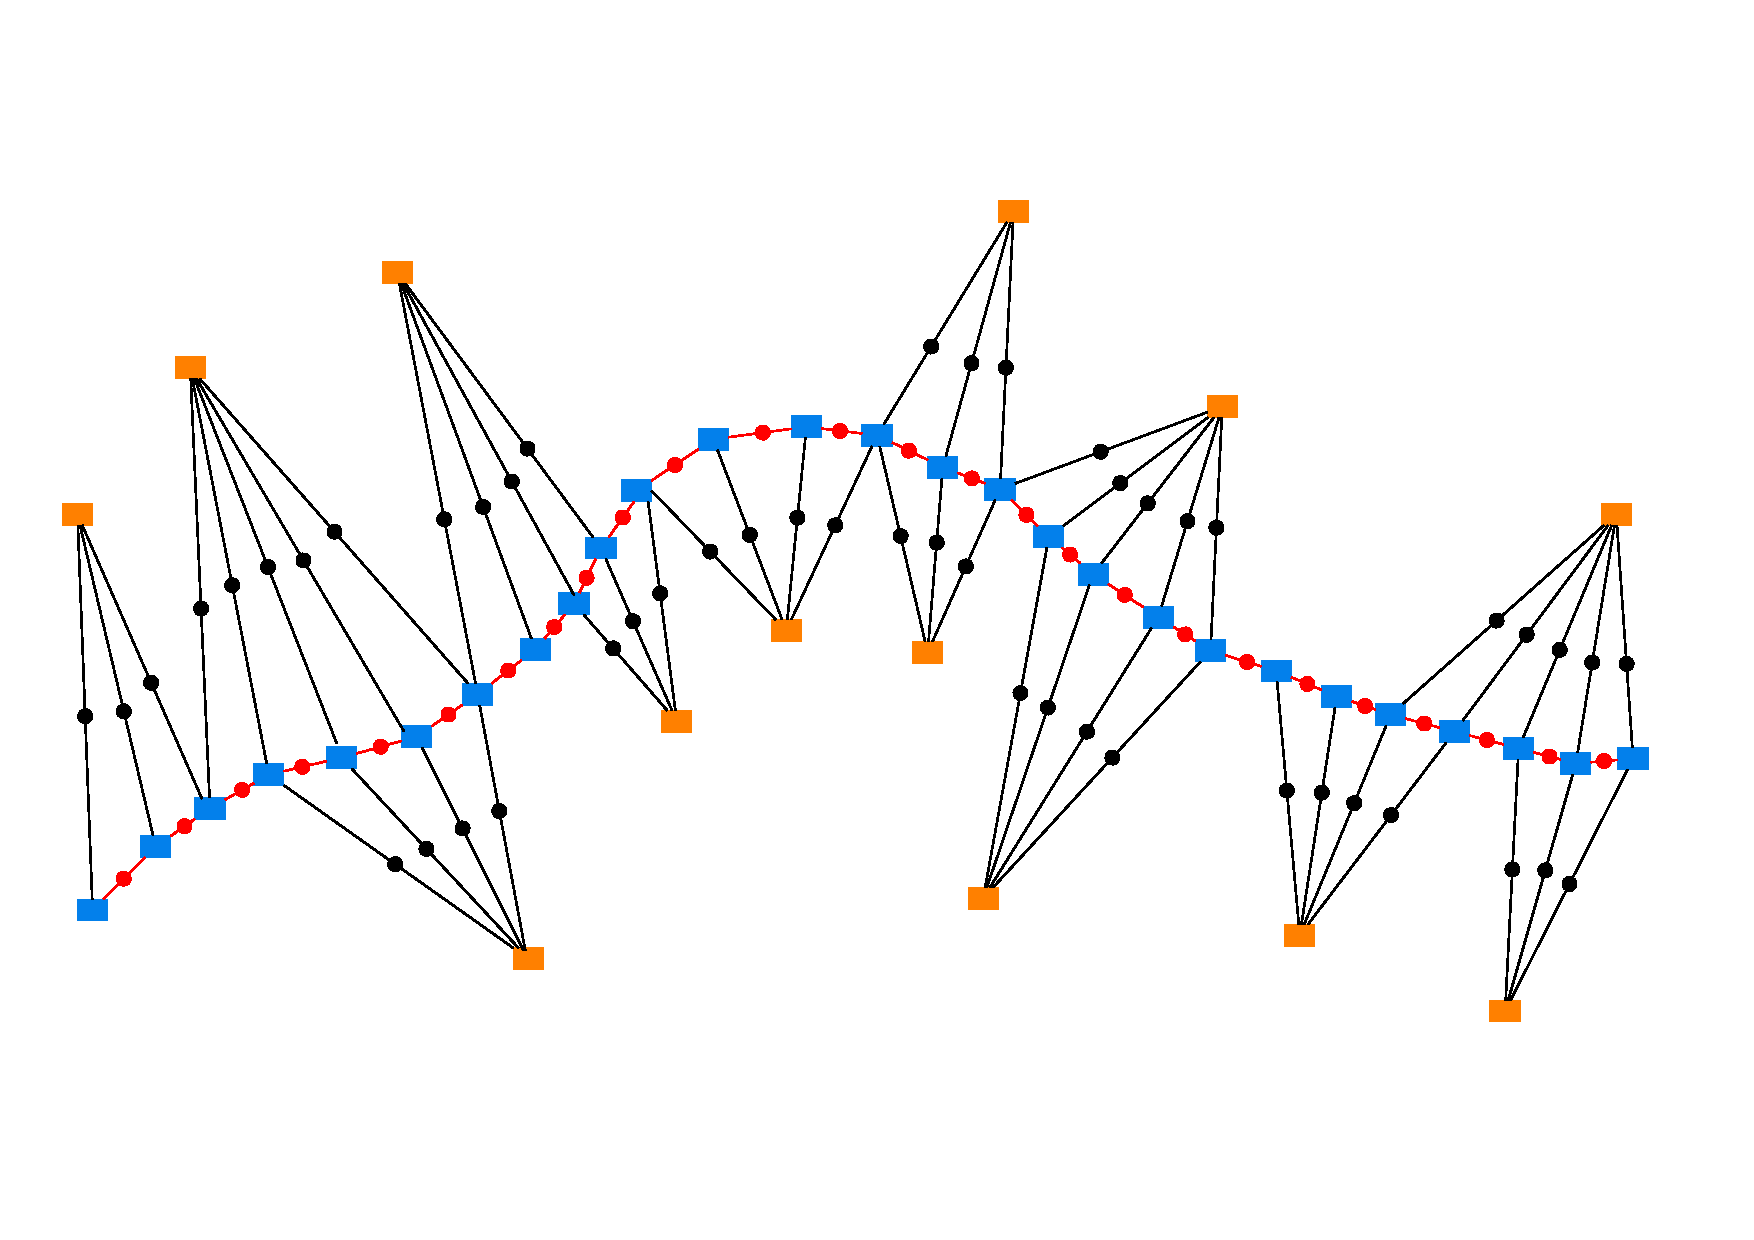
\includegraphics[width=\textwidth]{figures/02_basics/factor_graph.pdf}
    \caption{\textbf{Generic Factor Graph.} The figure depicts the structure of factor graph. The nodes are illustrated with colored squares and they can represent either a \textit{pose} - in blue - or a \textit{salient world point} - in orange. Measurements coming from the sensors are the constraints that connect the nodes, illustrated with circles - red for pose constraints and black for point ones.} 
    \label{fig:factor_graph}
\end{figure}

\section{Factor Graphs}\label{sec:factor_graph}
Until now, it has been showed the methodology to solve a least-squares minimization problem whose cost function is given by \ref{eq:cost_function}. In the previous Section, it has been underlined the \textit{sparsity} of the problem. In particular it has been stated that, given the state $\state = \left(\state_1, ..., \state_N\right)$, the measurement $\meas_k$ represents a \textbf{constraint} relating only a subset of the whole state vector, namely $\state_k = \left(\state_{k_1}, ..., \state_{k_q}\right) \subseteq \state = \left(\state_1, ..., \state_N\right)$. In this sense, the error $\error_k(\pred_k, \meas_k)$ describes how well the parameter blocks in $\state_k$ satisfy the constraint $\meas_k$ and, in fact, it is $\zero$ when $\state_k$ perfectly matches the constraint.

A problem that has this formulation, can be easily represented with a \textit{directed hyper-graph}, where

\begin{itemize}
    \item Each parameter block $\state_i \in \state_k$ represents a node $i$ in the hyper-graph
    \item Each constraint $\meas_k$ represents an hyper-edge that links all the nodes $\state_i \in \state_k$.
\end{itemize}

\noindent Obviously, when the hyper-edges have size $2$, the hyper-graph becomes an ordinary graph. Figure \ref{fig:factor_graph} shows the concept underlying this problem formulation.

Graph-based formulations are very common for the SLAM problem, since they help the optimization process and, in fact, most of the current state-of-the-art systems are based on this formulation. In fact, exploiting the \textit{topology} of the graph it is possible to achieve better performances, both in terms of speed and accuracy of the solution.

\vspace{15px}

Now that the underlying theory has been exploited, it is possible to better explain the typical formulations of the problem addressed in SLAM. Therefore, the next Chapter will propose an overview of the most common ones, in particular for 3D environments.